\documentclass[10pt,a4paper]{article}
\usepackage[bindingoffset=0.2in,%
            left=2.5cm,right=2cm,top=2.7cm,bottom=1in,%
            footskip=.25in]{geometry}
\usepackage[utf8]{inputenc}
\usepackage[ngerman]{babel}
\usepackage{amsmath, amsfonts, amssymb}
\usepackage{scrpage2}
\usepackage{color}
\usepackage{titlesec}
\pagestyle{scrheadings}
\usepackage{ulem, contour}
\usepackage{multicol}
\usepackage{hyperref}
\usepackage{pdfpages}
\usepackage{tabularx}
\usepackage{subcaption, float}
\usepackage{scrextend}
\usepackage{enumerate, enumitem}
\usepackage[bottom, splitrule]{footmisc}
\usepackage{multirow}
\usepackage{csquotes}

\usepackage[style=authoryear, backend=biber]{biblatex}
\addbibresource{bibliography.bib}

\renewcommand{\ULdepth}{1.8pt}
\contourlength{0.8pt}

\newcommand{\cul}[1]{%
  \uline{\phantom{#1}}%
  \llap{\contour{white}{#1}}%
}

\graphicspath{
    {Images/}
}

\makeatletter
\newcommand*{\rom}[1]{\expandafter\@slowromancap\romannumeral #1@}
\makeatother

\newrobustcmd*{\parentexttrack}[1]{%
  \begingroup
  \blx@blxinit
  \blx@setsfcodes
  \blx@bibopenparen#1\blx@bibcloseparen
  \endgroup}

\AtEveryCite{%
  \let\parentext=\parentexttrack%
  \let\bibopenparen=\bibopenbracket%
  \let\bibcloseparen=\bibclosebracket}

\definecolor{gray}{rgb}{0.33, 0.33, 0.33}
\definecolor{greengreen}{rgb}{0.0, 0.56, 0.0}
\definecolor{fgreen}{rgb}{0.13, 0.55, 0.13}
\definecolor{grellow}{rgb}{0.68, 1.0, 0.18}
\definecolor{orange}{rgb}{1.0, 0.49, 0.0}
\definecolor{deepblue}{rgb}{0,0,0.5}
\definecolor{deepred}{rgb}{0.6,0,0}
\definecolor{deepgreen}{rgb}{0,0.5,0}

\usepackage{pifont}

\newcommand{\cmark}{\ding{51}}%
\newcommand{\xmark}{\ding{55}}%
\newcommand{\wontfix}{\rlap{$\square$}{\large\hspace{1pt}\xmark}}


\newcommand{\vnr}{7}
\newcommand{\anr}{1}

\ihead{}
\ohead{Anfängerpraktikum 2}
\chead{Versuch \vnr, Abgabe \anr : \linebreak Elektrische Energie \& Wärmeenergie}
\cfoot{\pagemark}
\setheadsepline{.5pt}
\setlength\parindent{0pt}

\begin{document}

\begin{multicols}{2}
\begin{labeling}{Versuch-Nr.:}
\item[\textcolor{white}{x}Protokollant:\hspace{38pt}] \cul{Name} \wontfix
\item[\textcolor{white}{x}Zusammenarbeit\footnotemark mit:] \cul{Name} $\square$
\item[\textcolor{white}{x}Datum:\hspace{62pt}] \cul{\today}

\columnbreak

\item[Kurs: \hspace{27pt}] \cul{Anfängerpraktikum 2}
\item[Assistent: \hspace{8.7pt}] \cul{Name}
\item[Versuch-Nr.:] \underline{\vnr}
\end{labeling}
\end{multicols}

\begin{figure}[h]
\hspace{-0.5cm}\centerline{\includegraphics[width=1.1\linewidth , height=19cm]{Deckblatt_rest}}
\end{figure}

\newpage

\tableofcontents

\vspace{10pt}

\section{Aufgabenstellung}
\begin{flushleft}
Der Versuch \vnr \hspace{1pt}\glqq Umwandlung von elektrischer Energie in Wärmeengerie\grqq behandelt das Ermitteln der spezifischen Wärmekapazität von Stoffen. Genauer soll es um die Berechnung der spezifischen Wärmekapazität von Wasser gehen.
\end{flushleft}

\subsection{Physikalischer Hintergrund}
\begin{flushleft}
Die \textbf{spezifische Wärmeenergie} $c$ ist eine Stoffeigenschaft, die die Fähigkeit des Stoffes bemisst, Wärmeenergie zu speichern. \\

Wir können die Wärmeenergie dabei über die folgende Formel bestimmen:
\begin{equation}
Q = C \cdot (T_{Ende} - T_{Anfang})
\end{equation}
Dabei bezeichnet $C$ die Wärmekapazität, $Q$ die zugeführte Wärmeenergie und $T_{Ende}$ sowie $T_{Anfang}$ die Anfangs- und Endtemperatur. Die zugeführte Wärmeenergie kann dabei durch gut Messbare Größen bestimmt werden:
\begin{equation}\label{eq:qw}
Q = U \cdot I \cdot t
\end{equation}
Die spezifische Wärmekapazität kann darüber hinaus über die Masse berechnet werden.
\begin{equation}
c = \frac{C}{M}
\end{equation}
In diesem versuch benötigen wir für das Wasser auch ein Behältnis (Kalorimeter), wodurch jedoch ein Fehler entsteht, der herausgerechnet werden muss. Dies können wir über die Gesamtwärmekapazität und den Wasserwert erreichen.
\begin{align}
C &= C_{H_2O} + C_{Kal} \\
W &= \frac{C_{Kal}}{c_{H_2O}} \label{eq:wcc}
\end{align}
Hierbei gibt der Wasserwert an, wie viel Wasser unser Behälter ersetzt - wir berechnen also die Äquivalente Masse an Wasser für das Kalorimeter.

Durch Zusammenführen der bisherigen Formeln ergibt sich für die spezifische Wärmeenergie:
\begin{equation}\label{eq:spezwa}
c_{H_2O} = \frac{U \cdot I \cdot t}{(M + W) \cdot (T_{Ende} - T_{Anfang})}
\end{equation}
\\
Den Wasserwert können wir dabei über die Mischtemperatur von warmen und kaltem Wasser bestimmen.
\begin{equation}
C_{Kal} \cdot (T_3 - T_1) = c_{H_2O} \cdot m \cdot (T_2 - T_3)
\end{equation}
Mit Gleichung \ref{eq:wcc} folgt dann für den Wasserwert $W$:
\begin{equation}\label{eq:wwert}
W = m \cdot \frac{(T_2 - T_3)}{(T_3 - T_1)}
\end{equation}
\end{flushleft}

\section{Messmethoden}
\begin{flushleft}
Bei diesem Versuch nutzen wir ein Kalorimeter, um die spezifische Wärmekapazität des Wassers festzustellen. Dafür müssen wir jedoch zunächst den \textbf{Wasserwert} des Kalorimeters bestimmen.
\end{flushleft}

\subsection{Versuchsaufbau}
\begin{flushleft}
Für diesen Versuch \vnr benötigen wir folgende Materialien:
\begin{itemize}[itemsep=0.1pt]
\item Ein Kalroimeter
\item Ein Thermometer zum Messen der temperatur des Wassers
\item Eine Spannungsquelle
\item Ein Volt- und ein Amperemeter (bzw. zwei Multimeter) zur Messung von Strom und Spannung
\item Ein Schiebepotentiometer zum Regulieren und Variieren der Spannung
\end{itemize}
\end{flushleft}

\subsection{Schaltpläne}
\begin{figure}[h]
\centering
\includegraphics[scale=0.4]{Schaltbild_Wkapa}
\caption{Schaltbild zum Aufbau des Versuches.}
\label{fig:schalt}
\end{figure}

\begin{flushleft}
Der Schaltplan zeigt den Aufbau für die Messung zur spezifischen Wärmekapazität. Für die vorausgehenden Messungen zur Bestimmung des Wasserwertes des Kalorimeters benötigt es lediglich des Kalorimeters, Thermometers und Wasser.
\end{flushleft}

\section{Versuchsdurchführung}
\begin{flushleft}
Wir beginnen mit der Bestimmung des Wasserwertes des Kalroimeters. Wir führen fünf \textit{Leermessungen} am Kalorimeter durch (im Folgenden als \glqq Reihe\grqq bezeichnet). Dazu nehmen wir das Kalorimeter und Thermometer und bauen diese wie im Schaltplan auf (den Rest nicht). Anschließend füllen wir $100 ml$ kaltes Wasser in das Kalorimeter und warten, bis Wasser und Kalorimeter die gleiche Temperatur haben (Dies ist $T_1$). Diese messen und notieren wir. Danach entleeren wir das Kalorimeter und füllen es mit $100 ml$ heißem Wasser ($T_2$). Während des Abkühlprozesses notieren wir dann die Zeit, die vergangen ist, wenn sich das Wasser um je $0.1^{\circ}C$ abgekühlt hat. Anahnd dieser Messdaten können wir die Mischtemperatur ($T_3$) bestimmen (dies ist der Punkt, an dem die Temperatur langsamer abzufallen beginnt). \\

Nachdem wir nun den Wasserwert kennen, können wir die spezifische Wärmeenergie des Wasser bestimmen und die Schaltung nach dem Schaltplan aufbauen. Wir füllen wieder $100ml$ kaltes Wasser in das Kalorimeter. Anschließend schalten wir den Strom ein und erwärmen das Wasser auf eine vorher bestimmte Endtemperatur. Dies führen wir drei mal durch und notieren uns jedes mal Spannung, Stromstärke und ERwärmungszeit.
\end{flushleft}

\newpage

\section{Versuchsergebnisse}
\hypertarget{VersErg}{}

\begin{table}[h]
\centering
\centerline{
\begin{subtable}[t]{0.2\textwidth}
\centering
\subcaption{Reihe 1.}
\label{tab:r1}
\begin{tabular}{|c|c|}
\hline
$T_1 (^{\circ}C)$ & 18.9 \\
\hline
$T_2 (^{\circ}C)$ & 49.5 \\
\hline
\hline
\hline
$t (s)$ & $T (^{\circ}C)$ \\
\hline
216 & 45.9 \\ 
\hline
220 & 45.8 \\ 
\hline
224 & 45.7 \\ 
\hline
229 & 45.6 \\ 
\hline
234 & 45.5 \\ 
\hline
240 & 45.4 \\ 
\hline
247 & 45.3 \\ 
\hline
255 & 45.2 \\ 
\hline
263 & 45.1 \\ 
\hline
271 & 45 \\ 
\hline
314 & 44.5 \\ 
\hline
364 & 44 \\ 
\hline
417 & 43.5 \\ 
\hline
471 & 43 \\ 
\hline
530 & 42.5 \\ 
\hline
590 & 42 \\ 
\hline
652 & 41.5 \\ 
\hline
718 & 41 \\ 
\hline
792 & 40.5 \\ 
\hline
866 & 40 \\ 
\hline
\end{tabular}
\end{subtable}%
%
\begin{subtable}[t]{0.2\textwidth}
\centering
\subcaption{Reihe 2.}
\label{tab:r2}
\begin{tabular}{|c|c|}
\hline
$T_1 (^{\circ}C)$ & 19.6 \\
\hline
$T_2 (^{\circ}C)$ & 53.2 \\
\hline
\hline
\hline
$t (s)$ & $T (^{\circ}C)$ \\
\hline
45 & 49.8 \\ 
\hline
46 & 49.7 \\ 
\hline
50 & 49.6 \\ 
\hline
53 & 49.5 \\ 
\hline
57 & 49.4 \\ 
\hline
61 & 49.3 \\ 
\hline
66 & 49.2 \\ 
\hline
72 & 49.1 \\ 
\hline
79 & 49 \\ 
\hline
84 & 48.9 \\ 
\hline
90 & 48.8 \\ 
\hline
97 & 48.7 \\ 
\hline
104 & 48.6 \\ 
\hline
111 & 48.5 \\ 
\hline
\end{tabular}%
\end{subtable}
%
\begin{subtable}[t]{0.2\textwidth}
\centering
\subcaption{Reihe 3.}
\label{tab:r3}
\begin{tabular}{|c|c|}
\hline
$T_1 (^{\circ}C)$ & 19.4 \\
\hline
$T_2 (^{\circ}C)$ & 54.4 \\
\hline
\hline
\hline
$t (s)$ & $T (^{\circ}C)$ \\
\hline
36 & 50.3 \\ 
\hline
37 & 50.2 \\ 
\hline
39 & 50.1 \\ 
\hline
42 & 50 \\ 
\hline
46 & 49.9 \\ 
\hline
51 & 49.8 \\ 
\hline
56 & 49.7 \\ 
\hline
61 & 49.6 \\ 
\hline
67 & 49.5 \\ 
\hline
73 & 49.4 \\ 
\hline
\end{tabular}
\end{subtable}%
%
\begin{subtable}[t]{0.2\textwidth}
\centering
\subcaption{Reihe 4.}
\label{tab:r4}
\begin{tabular}{|c|c|}
\hline
$T_1 (^{\circ}C)$ & 19.6 \\
\hline
$T_2 (^{\circ}C)$ & 65.4 \\
\hline
\hline
\hline
$t (s)$ & $T (^{\circ}C)$ \\
\hline
35 & 60 \\ 
\hline
39 & 59.9 \\ 
\hline
41 & 59.8 \\ 
\hline
43 & 59.7 \\ 
\hline
45 & 59.6 \\ 
\hline
47 & 59.5 \\ 
\hline
50 & 59.4 \\ 
\hline
53 & 59.3 \\ 
\hline
55 & 59.2 \\ 
\hline
58 & 59.1 \\ 
\hline
61 & 59 \\ 
\hline
64 & 58.9 \\ 
\hline
67 & 58.8 \\ 
\hline
70 & 58.7 \\ 
\hline
74 & 58.6 \\ 
\hline
78 & 58.5 \\ 
\hline
82 & 58.4 \\ 
\hline
85 & 58.3 \\ 
\hline
89 & 58.2 \\ 
\hline
93 & 58.1 \\ 
\hline
\end{tabular}%
\end{subtable}
%
\begin{subtable}[t]{0.2\textwidth}
\centering
\subcaption{Reihe 5.}
\label{tab:r5}
\begin{tabular}{|c|c|}
\hline
$T_1 (^{\circ}C)$ & 20.9 \\
\hline
$T_2 (^{\circ}C)$ & 60.4 \\
\hline
\hline
\hline
$t (s)$ & $T (^{\circ}C)$ \\
\hline
55 & 55.6 \\ 
\hline
59 & 55.5 \\ 
\hline
61 & 55.4 \\ 
\hline
64 & 55.3 \\ 
\hline
67 & 55.2 \\ 
\hline
70 & 55.1 \\ 
\hline
73 & 55 \\ 
\hline
77 & 54.9 \\ 
\hline
80 & 54.8 \\ 
\hline
85 & 54.7 \\ 
\hline
89 & 54.6 \\ 
\hline
94 & 54.5 \\ 
\hline
98 & 54.4 \\ 
\hline
102 & 54.3 \\ 
\hline
108 & 54.2 \\ 
\hline
113 & 54.1 \\ 
\hline
117 & 54 \\ 
\hline
\end{tabular}
\end{subtable}%
}

\caption{Messergebnisse zur Berechnung des Wasserwertes.}
\label{tab:reihen}
\end{table}
\textit{Hinweis}: Der absolute Fehler der Temperaturen ist für alle Einträge mit $\Delta T = 0.1 ^{\circ}C$ angegeben.

\begin{figure}[H]
\centering
\begin{subfigure}[c]{.5\textwidth}
\centering
\includegraphics[scale=0.3]{Reihe1}
\subcaption{Graphsiche Darstellung der Ergebnisse \linebreak von Reihe 1.}
\label{fig:r1}
\end{subfigure}%
%
\begin{subfigure}[c]{.5\textwidth}
\centering
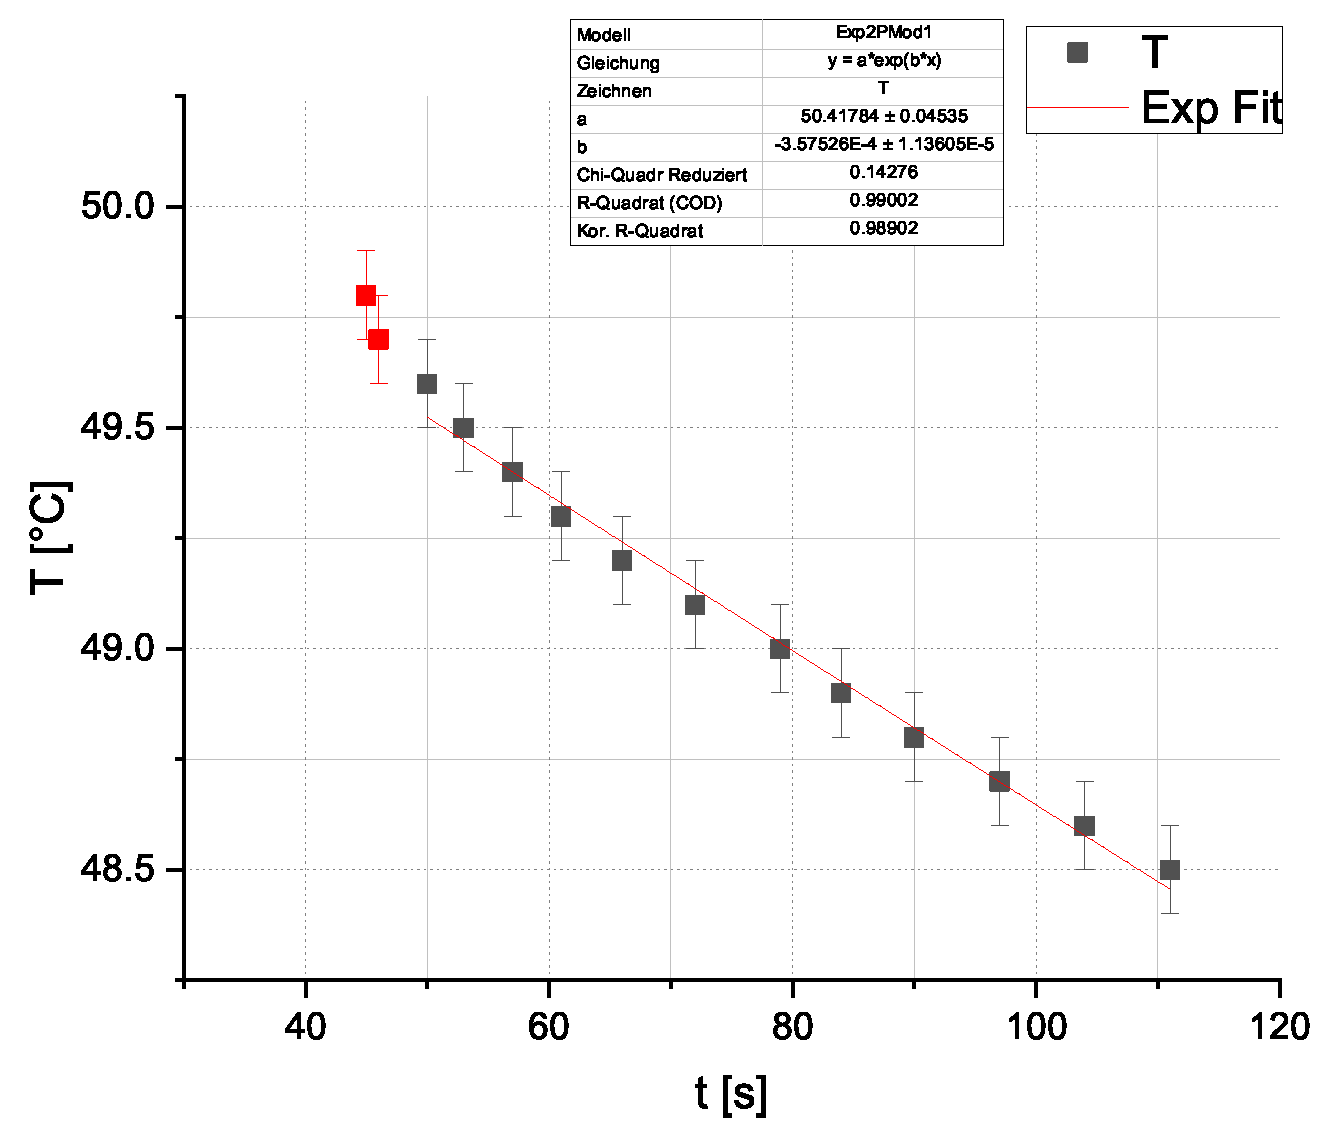
\includegraphics[scale=0.3]{Reihe2}
\subcaption{Graphsiche Darstellung der Ergebnisse \linebreak von Reihe 2.}
\label{fig:r2}
\end{subfigure}%

\begin{subfigure}[c]{.5\textwidth}
\centering
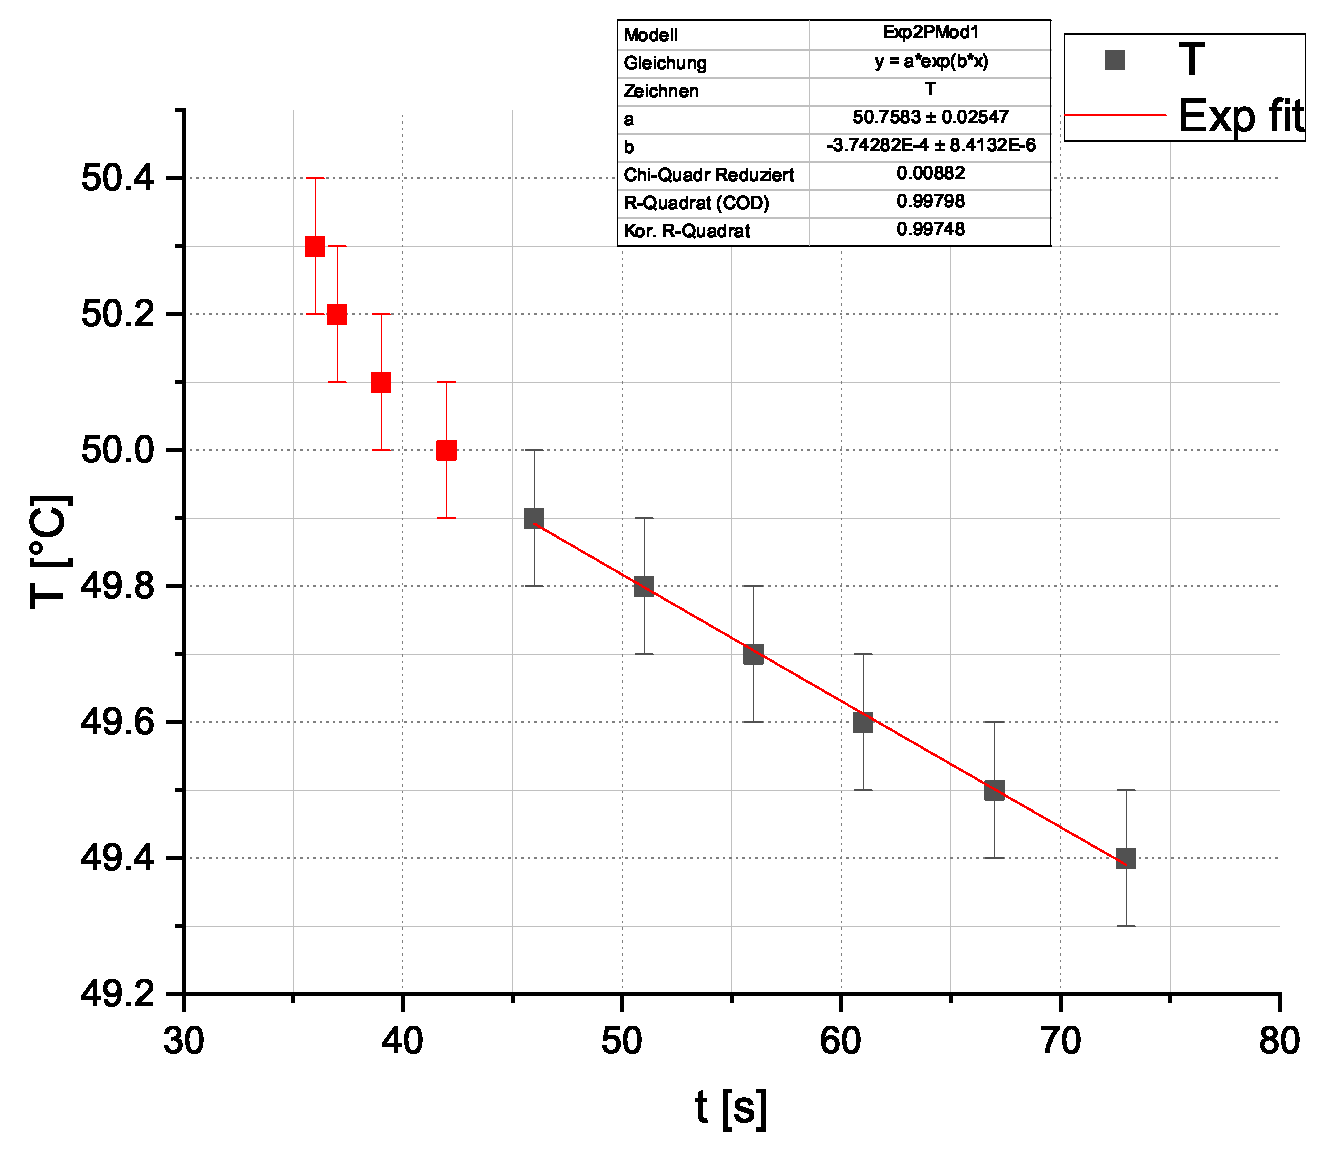
\includegraphics[scale=0.3]{Reihe3}
\subcaption{Graphsiche Darstellung der Ergebnisse \linebreak von Reihe 3.}
\label{fig:r3}
\end{subfigure}%
%
\begin{subfigure}[c]{.5\textwidth}
\centering
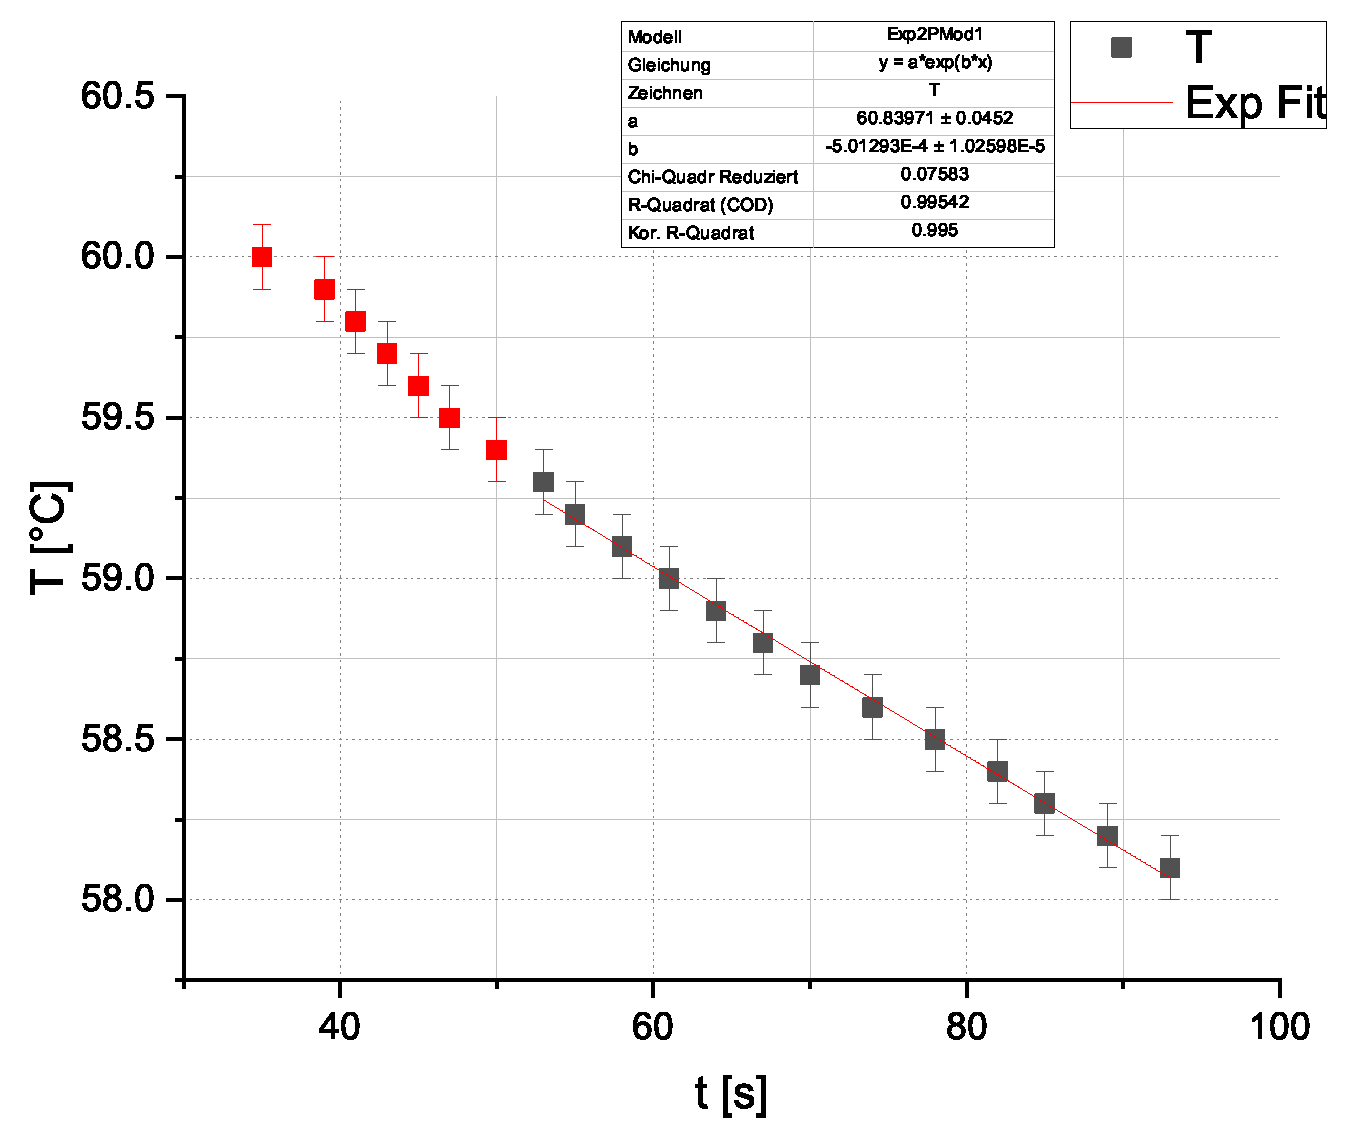
\includegraphics[scale=0.3]{Reihe4}
\subcaption{Graphsiche Darstellung der Ergebnisse \linebreak von Reihe 4.}
\label{fig:r4}
\end{subfigure}%

\begin{subfigure}[c]{.5\textwidth}
\centering
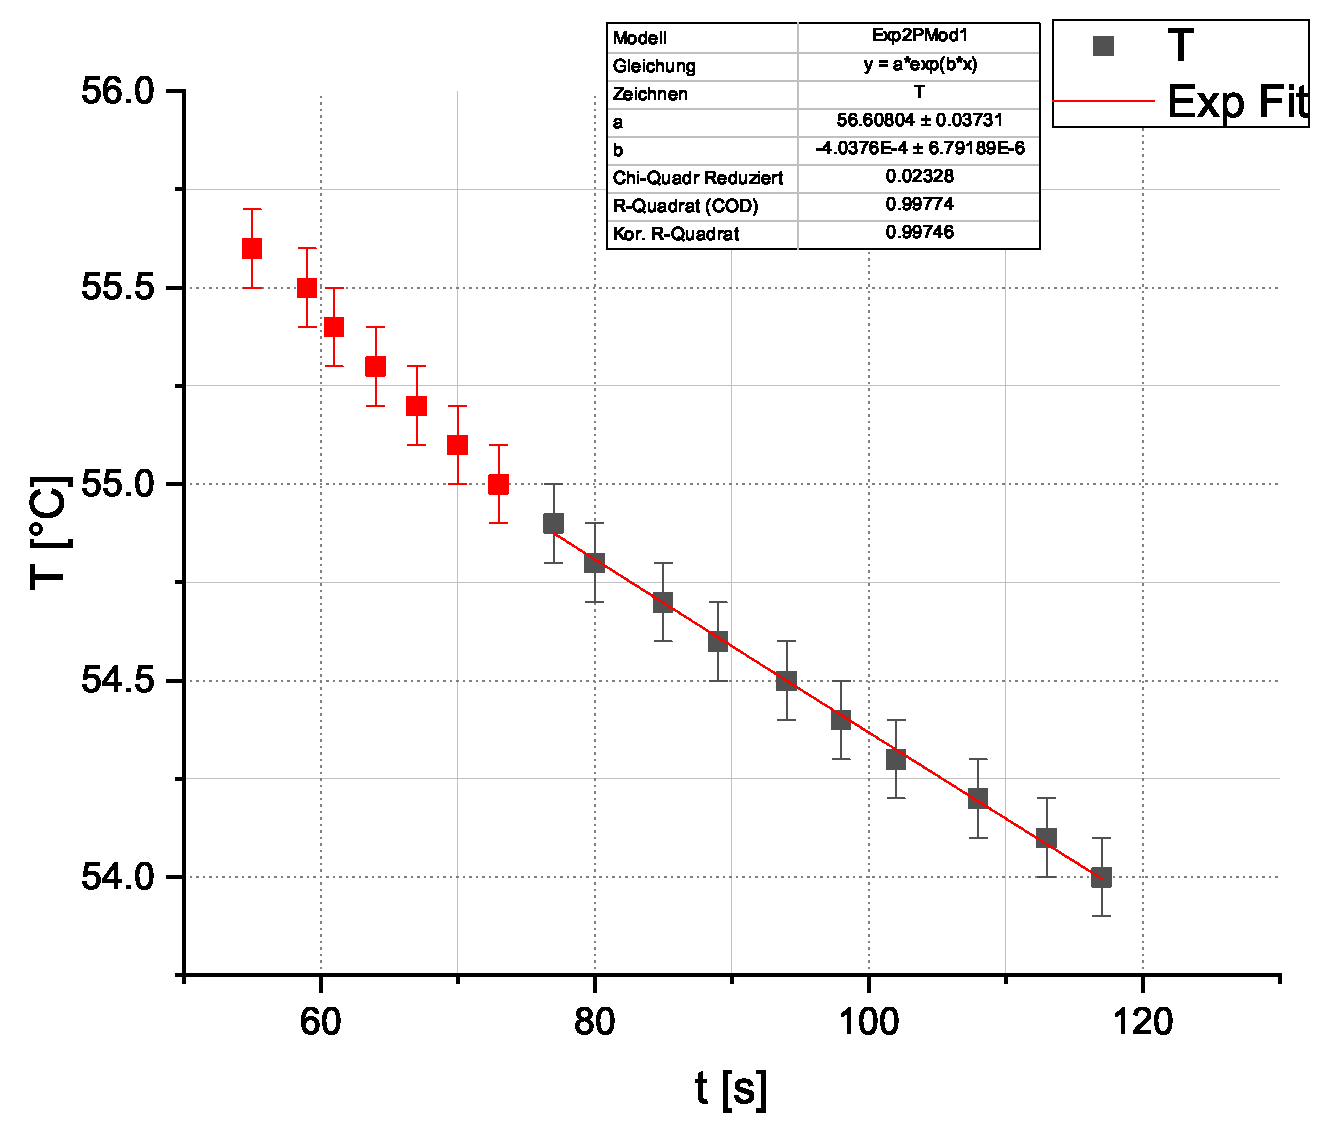
\includegraphics[scale=0.3]{Reihe5}
\subcaption{Graphsiche Darstellung der Ergebnisse \linebreak von Reihe 5.}
\label{fig:r5}
\end{subfigure}%
\caption{Graphische Darstellung der Messergebnisse zum Wasserwert.}
\label{fig:reihen}
\end{figure}

\begin{flushleft}
Die Tabelle(n) \ref{tab:reihen} und Abbildung(en) \ref{fig:reihen} zeigen die Messergebnisse zur Bestimmung des Wasserwertes des Kalroimeters nach Schaltplan (Abbiludng \ref{fig:schalt}). Aus diesen Ergebnissen können wir nun die benötigte Temperatur $T_3$ ablesen und den Wasserwert bestimmen (Gleichung \ref{eq:wwert}). Wir haben bei jeder Reihe $100ml = 100g$ Wasser verwendet.
\end{flushleft}
\begin{align*}
T_3(R_1) &= 45^{\circ}C & T_3(R_2) &= 49.6^{\circ}C & T_3(R_3) &= 49.9^{\circ}C & T_3(R_4) &= 59.3^{\circ}C & T_3(R_5) &= 54.9^{\circ}C
\end{align*}
\begin{align*}
W_{R_1} &= 100g \cdot \frac{49.5^{\circ}C - 45^{\circ}C}{45^{\circ}C - 18.9^{\circ}C} = \frac{500}{29}g \approx 17.2414g \\
W_{R_2} &= 100g \cdot \frac{53.2^{\circ}C - 49.6^{\circ}C}{49.6^{\circ}C - 19.6^{\circ}C} = 12g \\
W_{R_3} &= 100g \cdot \frac{54.4^{\circ}C - 49.9^{\circ}C}{49.9^{\circ}C - 19.4^{\circ}C} = \frac{900}{61}g \approx 14.7541g \\
W_{R_4} &= 100g \cdot \frac{65.4^{\circ}C - 59.3^{\circ}C}{59.3^{\circ}C - 19.6^{\circ}C} = \frac{6100}{397}g \approx 15.3652g \\
W_{R_5} &= 100g \cdot \frac{60.4^{\circ}C - 54.9^{\circ}C}{54.9^{\circ}C - 20.9^{\circ}C} = \frac{1050}{29}g \approx 16,1765g \\
\end{align*}
\begin{flushleft}
Aus diesen Berechneten Werten für den Wasserwert bestimmen wir den Mittelwert. Diesen verwenden wir für die weiteren Berechnungen zur spezifischen Wärmekapazität.
\end{flushleft}
\begin{figure}[H]
\centering
\begin{subfigure}[t]{.5\textwidth}
\centering
\begin{align*}
\varnothing W &= \frac{\sum W_{R_i}}{n} \\
&= \frac{75.5372}{5}g \\
&\approx 15.10744g
\end{align*}
\end{subfigure}%
%
\begin{subfigure}[t]{.5\textwidth}
\centering
\begin{align*}
\sigma_{\bar{x}} &= \frac{\sigma}{\sqrt{n}} = \sqrt{\frac{\sum(W_{R_i} - \varnothing W)^2}{n-1}} \cdot \frac{1}{\sqrt{n}} \\
&= \sqrt{\frac{15.54414729}{4}} \cdot \frac{1}{\sqrt{5}}g \\
&\approx 0.8815937g
\end{align*}
\end{subfigure}%
\end{figure}
\begin{flushleft}
Der Wasserwert des Kalorimeters beträgt somit $(15.11 \pm 0.88)g$.
\end{flushleft}

\begin{table}[h]
\centering
\caption{Messergebnisse zur Berechnugn der spezifischen Wärmekapazität (Siehe auch: Gleichung \ref{eq:spezwa}).}
\footnotesize
\centerline{
\begin{tabular}{|c|c|c|c|c|c|c|c|c|c|c|c|c|c|}
\hline
$U (V)$ & $U_{max} (V)$ & $\Delta U (V)$ & $I (A)$ & $I_{max} (A)$ & $\Delta I (A)$ & $t (s)$ & $T_a (^{\circ}C)$ & $T_e (^{\circ}C)$ & $\Delta T (^{\circ}C)$ & $W (g)$ & $\Delta W (g)$ & $c_{H_2O} (kJ)$ & $\Delta c_{H_2O} (kJ)$ \\
\hline
30 & 60 & 1.2 & 1.55 & 3 & 0.06 & 84 & 21.7 & 30 & 0.1 & 15.11 & 0.88 & 4.089 & 0.087 \\ 
\hline
19 & 60 & 1.2 & 0.95 & 3 & 0.06 & 233 & 21.2 & 30 & 0.1 & 15.11 & 0.88 & 4.152 & 0.134 \\ 
\hline
26 & 60 & 1.2 & 1.35 & 3 & 0.06 & 133 & 20.1 & 30 & 0.1 & 15.11 & 0.88 & 4.097 & 0.099 \\ 
\hline
\end{tabular}
}
\normalsize
\end{table}
\begin{flushleft}
Wir haben nun drei Messungen zur Bestimmung des Wasserwertes durchgeführt. Wir berechnen wie auch zuvor beim Wasserwert wieder den Mittelwert der spezifischen Wärmekapazitäten.
\end{flushleft}
\begin{figure}[H]
\centering
\begin{subfigure}[t]{.5\textwidth}
\centering
\begin{align*}
\varnothing c &= \frac{\sum c_i}{n} \\
&= \frac{12.33657}{3} kJ \\
&\approx 4.11219 kJ
\end{align*}
\end{subfigure}%
%
\begin{subfigure}[t]{.5\textwidth}
\centering
\begin{align*}
\sigma_{\bar{x}} &= \frac{\sigma}{\sqrt{n}} = \sqrt{\frac{\sum(c_i - \varnothing c)^2}{n-1}} \cdot \frac{1}{\sqrt{n}} \\
&= \sqrt{\frac{2.3533483 \cdot 10^{-3}}{2}} \cdot \frac{1}{\sqrt{3}} kJ \\
&\approx 0.01980466 kJ
\end{align*}
\end{subfigure}%
\end{figure}
\begin{flushleft}
Der Versuch bringt uns somit auf einen Wert von $c_{H_2O} = (4.11 \pm 0.02)kJ$.
\end{flushleft}

\subsection{Diskussion der Messergebnisse}
\begin{flushleft}
Der Literaturwert der spezifischen Wärmekapazität von Wasser beläuf sich auf $4.184 kJ$ (bei $20^{\circ}C$)\footnote{Siehe: \href{https://de.wikipedia.org/wiki/Spezifische_W\%C3\%A4rmekapazit\%C3\%A4t}{Quelle (Wikipedia)}}. Der von uns berechnete Wert ($c_{H_2O} = (4.11 \pm 0.02)kJ$) weicht um ca. $0.074 kJ$ bzw. $1.77\%$ ab. Dies ist ein recht genaues Ergebnis.
\end{flushleft}
\begin{flushleft}
Im weiteren wollen wir die \textbf{Halbwertszeit} des Kalorimeters ermitteln. Diese gibt an, nach welcher Zeit die Temperatur auf die Hälfte des Anfangswertes abgesunken ist. Dafür haben wir in den Graphen zur ERmittlung des Wasserwertes (Abilldung \ref{fig:reihen}) einen exponentiellen Fit vorgenommen. Dabei ist zu erkennen, dass die Werte zwischen Graph \ref{fig:r1} zu Reihe eins und den Graphen zu den restlichen Reihen relativ stark abweicht. Die Ursache liegt dabei beim Überwachungszeitraum, der bei den Reihen zwei bis fünf viel geringer ist, als bei Reihe eins. Aus diesem Grund verwenden wir zur Berechnung der Halbwertszeit die Werte aus dem Fit von Graph \ref{fig:r1}.

Wir haben somit also die Funktion der Temperatur:
\begin{equation}\label{eq:expotemp}
f_{temp}(t) = 47.175 \cdot e^{-t \cdot 1.94 \cdot 10^{-4}}
\end{equation}
Konkret berechnet sich die Halbwertszeit dann mit $f_{temp}(t_H) = \frac{46}{2} = 23 [^{\circ}C]$.
\begin{align*}
f_{temp}(t) &= 47.175 \cdot e^{-t \cdot 1.94 \cdot 10^{-4}} \\
\frac{f_{temp}(t)}{47.175} &= e^{-t \cdot 1.94 \cdot 10^{-4}} \\
ln \left( \frac{f_{temp}(t)}{47.175} \right) &= -t \cdot 1.94 \cdot 10^{-4} \\
t_H &= - ln \left( \frac{f_{temp}(t_H)}{47.175} \right) \cdot \frac{1}{1.94 \cdot 10^{-4}} \\
t_H &= - ln \left( \frac{23}{47.175} \right) \cdot \frac{1}{1.94 \cdot 10^{-4}} \\
t_H &\approx 3702.884 s \approx 61.715 min
\end{align*}
Die Halbwertszeit des Kalorimeter beläuft sich auf etwa \textit{eine Stunde}.
\end{flushleft}
\begin{flushleft}
Zuletzt stellt sich noch die Frage, welche Auswirkungen die Nutzung des Wechselstroms bei dem Versuch aufweist. Dazu betrachten wir die Phasenverschiebung zwischen Strom und Spannung an der Heizspirale. Diese Überprüfung ist wichtig, um zu zeigen, das unsere Berechnungen (bzw. Formeln) korrekt sind.
\begin{figure}[H]
\centering
\includegraphics[scale=0.5]{screen_phasen}
\caption{Phasen von Strom (blau) und Spannung (gelb).}
\label{fig:phasen}
\end{figure}
Wie Abbildung \ref{fig:phasen} zeigt, sind Strom und Spannung in Phase, wodurch gilt:
\begin{align*}
W &= U_{eff} \cdot I_{eff} \cdot t \cdot cos(90^{\circ}) \\
W &= U_{eff} \cdot I_{eff} \cdot t
\end{align*}
Somit fällt zu jedem Zeitpunkt die gesamte Arbeit an der Heizspirale ab. Somit ist die Formel \ref{eq:qw} korrekt verwendet worden.
\end{flushleft}

\section{Fazit}
\begin{flushleft}
Der Versuch \vnr\hspace{1pt} hat gezeigt, dass man die spezifische Wärmekapazität von Flüssigkeiten berechnen kann, indem man das Behältnis der Flüssigkeit quasi in der Flüssigkeit aufwiegt.
\end{flushleft}

\begingroup
\raggedright
\sloppy
\printbibliography[heading=bibintoc,title={6 \hspace{6pt} Literatur}]
\endgroup
\end{document}
